%_____________________________________________________________________________________________ 
% Chapter 2: Background
%_____________________________________________________________________________________________ 
\chapter{Background}
\label{sec:background}

\section{System Model}

We assume the standard partially synchronous model of Dwork
et~al.~\cite{dls1988}: $n$ replicas, up to $f$ of which may be
Byzantine (arbitrary behaviour, including collusion), with
$n \ge 3f{+}1$.  Messages are eventually delivered once the network
stabilises, but there are no guarantees during asynchronous periods.
This model is the baseline for most modern BFT work, including
HotStuff, so we adopt it without modification.

\smallskip\noindent\textbf{Cluster-size restriction.}\quad
While the general BFT lower bound is $n \ge 3f{+}1$,
\persisthotstuff{} additionally requires $n \equiv 1 \pmod{3}$,
yielding valid cluster sizes $n \in \{4, 7, 10, 13, \ldots\}$.  For any
such $n$ the fault threshold is exactly $f = (n{-}1)/3$, so the
condition collapses to a tight equality $n = 3f{+}1$ rather than a
lower bound.

\section{How HotStuff Works}

We briefly recap the mechanics since our design builds directly on
them.  \hotstuff{}~\cite{hotstuff2019} runs in \emph{views}.  Each
view has a leader who does three things: proposes a block which
contains the command that needs to be executed, collects at least
$2f{+}1$ signed votes into a Quorum Certificate (QC), and broadcasts
the QC.  Safety comes from the \emph{3-chain commit rule}: a
block~$B_0$ is considered committed only when there is a chain
$B_0 \leftarrow B_1 \leftarrow B_2$ in which both $B_1$ and $B_2$
carry valid QCs.  Until that chain forms, $B_0$ is not executed.

The protocol's appeal is its simplicity.  Every decision costs $O(n)$
messages (one broadcast from the leader, $n{-}1$ votes back, one QC
broadcast).  If the leader is honest and the network is behaving, the
system moves at actual network speed rather than waiting for timeouts.
Fig.~\ref{fig:3chain_commit} illustrates the 3-chain structure.

\begin{figure}[t]
\centering
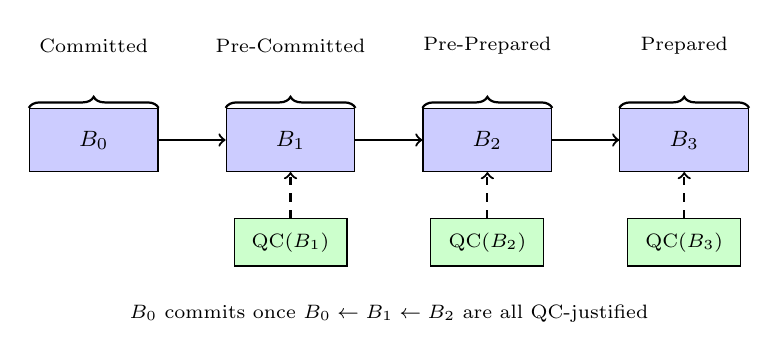
\begin{tikzpicture}
\tikzstyle{block}=[rectangle, draw, fill=blue!20, text width=1.4cm,
  text centered, minimum height=0.8cm, font=\footnotesize]
\tikzstyle{qc}=[rectangle, draw, fill=green!20, text width=1.2cm,
  text centered, minimum height=0.6cm, font=\scriptsize]
\tikzstyle{arrow}=[->, thick]

\node (B0) at (0,0)   [block] {$B_0$};
\node (B1) at (2.5,0) [block] {$B_1$};
\node (B2) at (5,0)   [block] {$B_2$};
\node (B3) at (7.5,0) [block] {$B_3$};

\node (QC1) at (2.5,-1.3) [qc] {QC($B_1$)};
\node (QC2) at (5,-1.3)   [qc] {QC($B_2$)};
\node (QC3) at (7.5,-1.3) [qc] {QC($B_3$)};

\draw [arrow] (B0) -- (B1);
\draw [arrow] (B1) -- (B2);
\draw [arrow] (B2) -- (B3);
\draw [arrow, dashed] (QC1) -- (B1);
\draw [arrow, dashed] (QC2) -- (B2);
\draw [arrow, dashed] (QC3) -- (B3);

\node[font=\scriptsize] at (0,   1.2) {Committed};
\draw [decorate,decoration={brace,amplitude=4pt},thick,yshift=3pt]
  (B0.north west) -- (B0.north east);
\node[font=\scriptsize] at (2.5, 1.2) {Pre-Committed};
\draw [decorate,decoration={brace,amplitude=4pt},thick,yshift=3pt]
  (B1.north west) -- (B1.north east);
\node[font=\scriptsize] at (5,   1.2) {Pre-Prepared};
\draw [decorate,decoration={brace,amplitude=4pt},thick,yshift=3pt]
  (B2.north west) -- (B2.north east);
\node[font=\scriptsize] at (7.5, 1.2) {Prepared};
\draw [decorate,decoration={brace,amplitude=4pt},thick,yshift=3pt]
  (B3.north west) -- (B3.north east);

\node[font=\scriptsize] at (3.75, -2.2)
  {$B_0$ commits once $B_0 \leftarrow B_1 \leftarrow B_2$
   are all QC-justified};
\end{tikzpicture}
\caption{The 3-chain commit rule.  $B_0$ is only safe to commit once two
  successive QC-justified blocks extend it.}
\label{fig:3chain_commit}
\end{figure}
